

Ce chapitre présente nos principaux résultats sur l'apprentissage et la correction 
des odométries proprioceptive et prédictive.
Tout d'abord, l'amélioration de précision apportée par l'utilisation 
des capteurs de pression est présentée.
Ensuite, deux études expérimentent sur le petit robot humanoïde Sigmaban
certains principes déjà appliqués aux robots à roues.
Dans la première étude, une technique de régression non paramétrique est employée
ainsi qu'un système de capteurs externes mesurant la pose absolue 
du robot pendant son déplacement.
Une comparaison approfondie de deux surfaces de marche est alors menée.
Ce système étant trop encombrant pour être déployé dans un contexte RoboCup,
la deuxième étude propose une méthode plus opérationnelle et permettant 
de se passer de ce dispositif externe. 
Ceci grâce à un modèle de correction linéaire et une méthode d'optimisation en boite noire.
Enfin, l'application à la planification du déplacement du robot est présentée.

\section{Définitions et motivations\label{sec:odometry_intro}}

Deux notions proches sont ici abordées et étudiées :
\begin{definition}
    L'\textit{odométrie proprioceptive} est l'estimation 
    du déplacement relatif du robot
    dans le monde à partir des informations des capteurs 
    internes du robot enregistrées au cours du déplacement.
    Le calcul ne se base pas sur la reconnaissance 
    de points de repères externes au robot.
    L'odométrie se calcule a posteriori pendant et après 
    le mouvement physique du robot.
    \footnote{Cette définition de l'odométrie n'inclue pas les méthodes 
    d'odométries visuelles se basant sur le suivi de
    points d'intérêts externe, même sans détecter de balises 
    de repérage dont la position est connue dans le repère du monde.}
\end{definition}
\begin{definition}
    Le \textit{modèle de déplacement} ou \textit{odométrie prédictive} 
    est l'estimation du déplacement relatif possible du robot
    dans le monde sous l'action d'une séquence d'ordres moteurs donnée. 
    Il s'agit d'une simulation a priori du déplacement du robot qui
    ne nécessite aucune action physique.
\end{definition}
À noter que les déplacements se représentent dans plan en position et 
en orientation comme décrit à la section \ref{sec:def_odometry}.\\

Une application importante du calcul de l'odométrie proprioceptive tient 
en la localisation du robot dans le monde
(un exemple d'application est illustré sur la figure \ref{fig:monitoring}).
Pour se situer de manière absolue dans 
un environnement, il est nécessaire d'y repérer des éléments extérieurs dont 
la position est connue ; dans notre cas à l'aide d'une caméra
et de techniques d'analyses d'images\footnote{
Les méthodes de visions mises en oeuvre par l'équipe Rhoban 
pour la RoboCup 2016 et 2017 sont présentées 
dans \cite{ChampionPaperRoboCup2016} et \cite{TDPRoboCup2017}}.
Une fois un point de repère reconnu, sa position relative dans
le repère égocentrique du robot est précisément évaluée.
Un calcul géométrique ou une accumulation des observations 
par filtre de Kalman ou filtre particulaire peuvent alors être employés 
pour en déduire la position absolue du robot dans le monde.

L'estimation de l'odométrie proprioceptive du robot est une composante
essentielle des méthodes de localisation.
L'odométrie peut en effet être intégrée à une fréquence souvent
bien plus élevée\footnote{La mise à jour à haute 
fréquence de l'odométrie est plus difficile avec les techniques d'odométries visuelles.}
que la localisation absolue se basant sur
l'analyse d'images de points de repères extérieurs.
En l'absence d'observation de repérage pendant plusieurs pas, 
l'odométrie permet de continuer à mettre à jour la pose du robot.
De plus, si le point de départ du déplacement est connu, l'odométrie fournit 
une première estimation de positionnement dont la lente dérive est alors 
corrigée ponctuellement par prise d'informations externes.\\

A contrario, le modèle de déplacement (odométrie prédictive ou simulée) 
trouve son intérêt non pas dans la perception mais dans le contrôle de 
la locomotion du robot.
Typiquement, le mouvement de marche est sur nos robots
toujours imparfait.
Il y a un écart parfois important entre l'ordre de déplacement 
souhaité donné au mouvement de marche et le déplacement réel du robot 
dans le monde physique (voir section \ref{sec:walk}).
Le modèle de déplacement a pour objet de capturer la relation
entre ces deux déplacements ; à modéliser les imperfections
de la boucle de marche et des perturbations de l'environnement.

L'application naturelle de l'odométrie prédictive réside dans
la planification de la meilleure séquence de pas permettant d'atteindre 
une certaine pose dans le monde.
La séquence d'ordres moteurs est optimisée au travers d'un simulateur
utilisant le modèle de déplacement du robot.
Ainsi, la solution de l'optimisation des ordres moteurs sera 
d'autant plus performante que le modèle de déplacement capture 
le comportement réel du robot.
La prise en compte des imperfections du déplacement du robot
améliore ainsi la partie boucle ouverte (pré commande) du contrôle 
de la locomotion.\\

Ces deux concepts sont fondamentalement proches et peuvent être 
construits au travers des mêmes méthodes et en utilisant les mêmes
données expérimentales.

\begin{figure}[htb]
    \begin{center}
        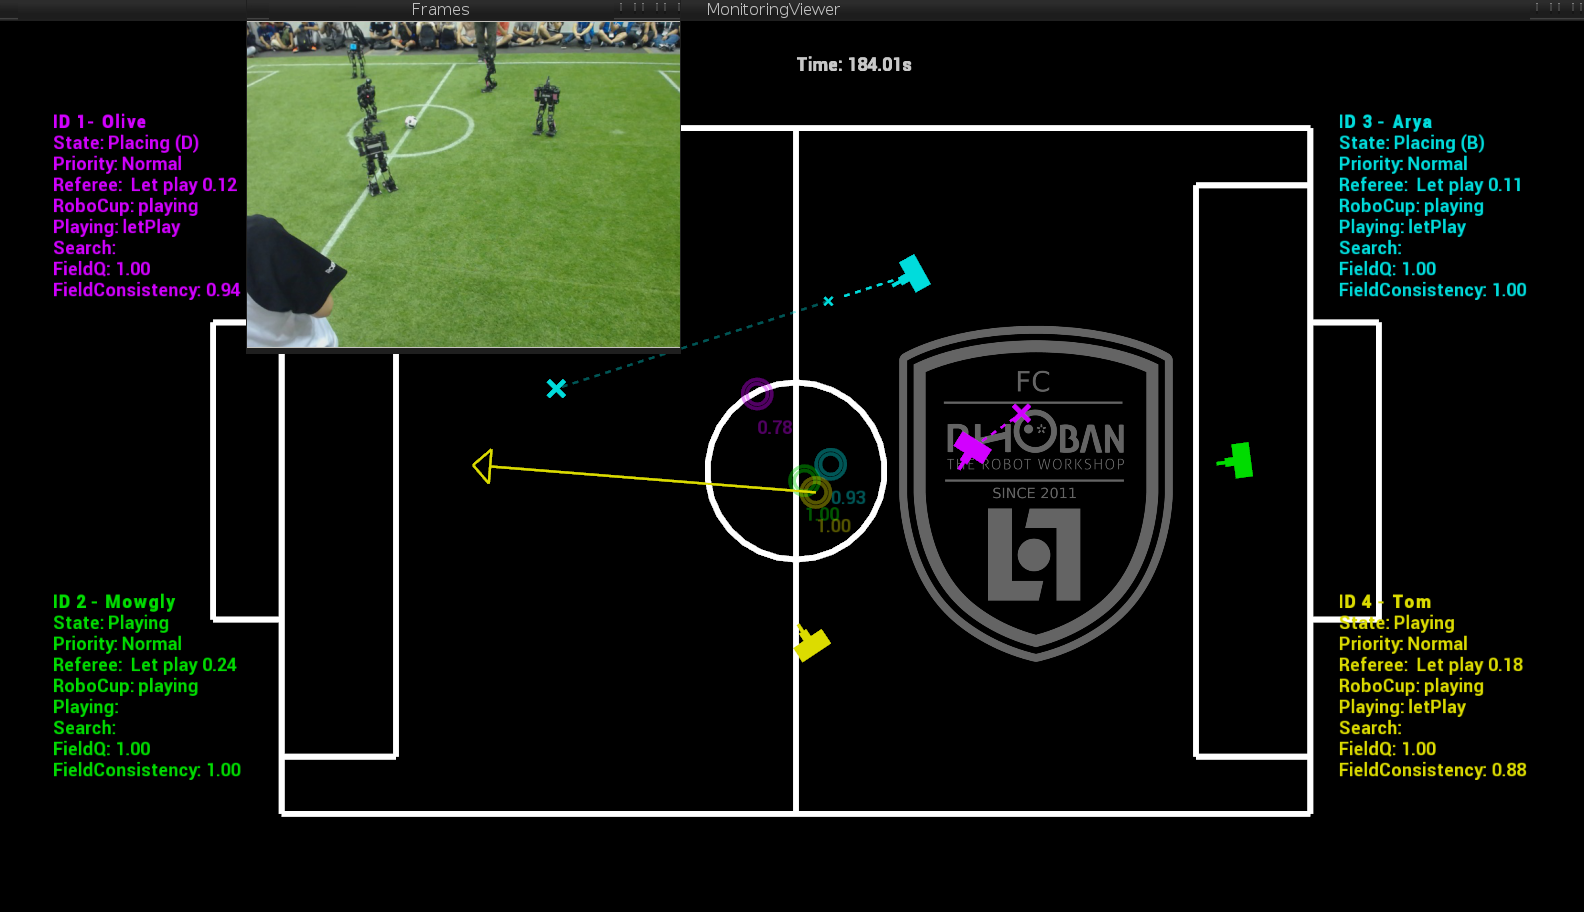
\includegraphics[width=1.0\linewidth]{../media/monitoring.png}
        \caption{\label{fig:monitoring} 
            Capture d'écran de l'outil graphique utilisé par l'équipe pour 
            surveiller en temps réel pendant les matchs l'état, la localisation 
            et les décisions stratégiques de tous les robots sur le terrain.
        }
    \end{center}
\end{figure}

\section{Utilisation des capteurs de pression\label{sec:odometry_pressure}}

Comme détaillé aux sections \ref{sec:estimation_etat} et \ref{sec:def_odometry},
la détection du changement de pied de support conditionne fortement
l'intégration du déplacement du robot au cours du temps.
Dans la méthode classique, le changement de pied de support
du modèle est déclenché par une condition géométrique : le pied le plus bas
dans le repère du monde est à tout instant considéré comme le pied de support.

Cependant, cette condition est peu robuste au bruit de l'IMU, même après filtrage.
De plus, cette méthode simple ne considère que le centre du pied. 
Il arrive souvent en pratique, à cause des jeux mécaniques et 
des défauts d'asservissement, que pendant la marche du robot, le pied
ne soit en contact avec le sol que sur une seule de ses arrêtes. 
Le centre du pied n'est alors plus sur le plan du sol ; influençant
la condition de hauteur de la transition.\\

L'utilisation des capteurs de pression sous les pieds du robot 
décrit à la section \ref{sec:robot_pressure_sensors} permet de grandement 
améliorer la précision de la détection du changement de pied de support.
Ces capteurs mesurent les forces verticales exercées sur chacun des quatre 
crampons situé aux coins des deux pieds.
Il est alors possible d'en déduire pour chaque pied la position
sur le sol du centre de pression (\textit{Center Of Pressure}, \textit{COP}) 
$\bm{p}_{\text{left}}^{\text{COP}},\bm{p}_{\text{right}}^{\text{COP}} \in \mathbb{R}^2$ ainsi 
que la répartition du poids du robot $w_{\text{left}}, w_{\text{right}}\in \mathbb{R}$ 
sur chacun des pieds.\\

En utilisant les capteurs de pression, la mise à jour
de l'état de support du robot donc est faite comme suit :
Si $w_{\text{left}} \geqslant w_{\text{right}}$ alors 
le pied gauche ($LSS$) est le pied de support, sinon il s'agit du pied droit ($RSS$). 
On considère donc ici que le pied sur lequel s'appuie le plus 
le robot est le pied fixe par rapport au sol.

\begin{figure}[htb]
    \begin{center}
        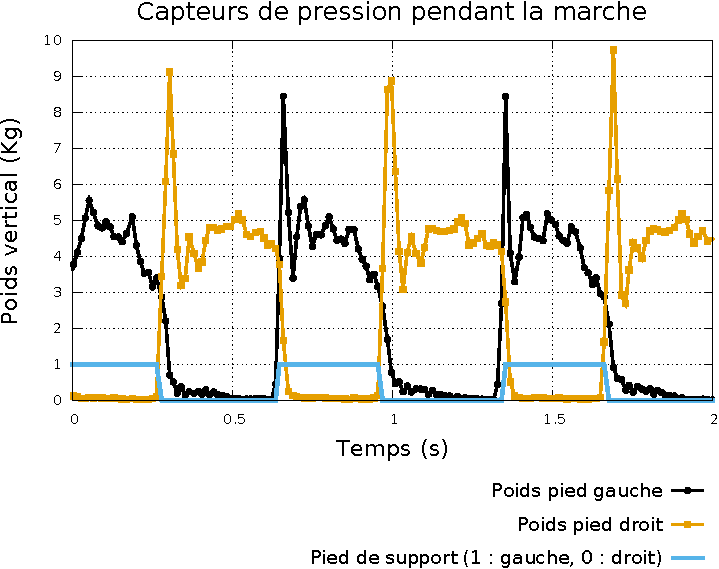
\includegraphics[type=pdf,ext=.pdf,read=.pdf,width=1.0\linewidth]{../plot/pressure_sensors}
        \caption{\label{fig:pressure_sensors} 
            Mesures des forces de pression verticales sur les pieds de Sigmaban
            alors que le robot marche vers l'avant (fréquence 1.7 Hz).
            La courbe bleue montre également le pied de support 
            courant gauche ou droit estimé.}
    \end{center}
\end{figure}

La figure \ref{fig:pressure_sensors} illustre le profil typique des mesures
de pression sur les deux pieds pendant un mouvement de marche ainsi
que le choix du pied de support courant.
À noter que le pic de pression observé au début de la phase d'appuis 
correspond à l'impact du pied avec le sol. Le poids total du robot 
valant $4.2$ Kg.\\

\begin{figure}[htb]
    \begin{center}
        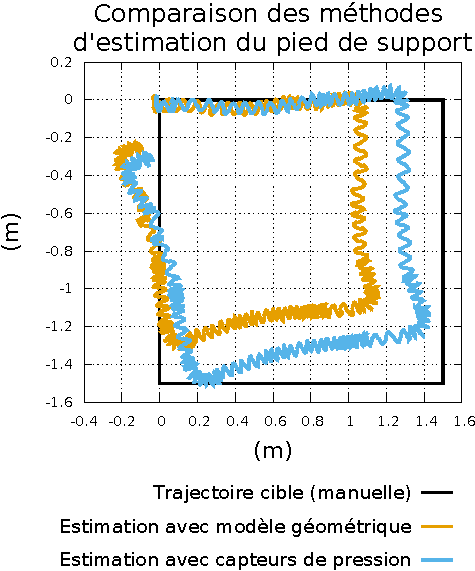
\includegraphics[type=pdf,ext=.pdf,read=.pdf,width=1.0\linewidth]{../plot/odometry_pressure_comparison}
        \caption{\label{fig:odometry_pressure_comparison} Comparaison de l'intégration
            de l'odométrie proprioceptive selon les deux méthodes d'estimation du pied support.
            Le robot Sigmaban est piloté manuellement pour marcher sur les bords 
            d'un carré de taille $1.5$ m et finit par revenir à sa position et
            orientation initiale.
        }
    \end{center}
\end{figure}

Enfin, la figure \ref{fig:odometry_pressure_comparison} illustre l'importance de l'estimation
du pied de support pour l'intégration de l'odométrie proprioceptive. 
Le robot est ici piloté manuellement pour suivre les quatre bords d'un carré de $1.5$ m de coté.
Le graphique montre l'odométrie estimée par le robot selon les deux critères d'évaluation du
pied de support courant ; en se basant sur la hauteur des pieds grâce au modèle géométrique direct
ou en se basant sur la répartition du poids sur chacun des pieds avec les capteurs de pression.

Quatre commentaires qualitatifs peuvent être tirés de ce graphique.
Une étude quantitative plus approfondie est développée dans la suite.
\begin{itemize}
    \item Les deux méthodes d'estimation de l'odométrie proprioceptive 
        tendent à sous estimer la distance réelle parcouru par le robot.
    \item L'utilisation des capteurs de pression améliore l'estimation des distances et
        la précision de l'odométrie.
    \item On observe distinctement la lente dérive de l'orientation basée sur l'intégration
        des gyromètres autour de la verticale.
    \item Malgré une nette différence d'estimation de la distance parcourue entre ces deux
        méthodes, la position finale atteinte est proche. À noter que les deux méthodes partagent 
        toutes deux la même estimation de l'orientation basée sur la centrale inertielle.
        Cet effet de \textit{repliement} montre que les trajectoires formant des boucles
        induisent des biais qu'il est important d'éviter autant que faire se peut.
        Si l'on ne compare que la position finale, on en déduit alors de manière 
        erronée que les deux méthodes ont des résultats similaires.
\end{itemize}

